% Template for Elsevier CRC journal article
% version 1.2 dated 09 May 2011

% This file (c) 2009-2011 Elsevier Ltd.  Modifications may be freely made,
% provided the edited file is saved under a different name

% This file contains modifications for Transportation Research Procedia

% Changes since version 1.1
% - added "procedia" option compliant with ecrc.sty version 1.2a
%   (makes the layout approximately the same as the Word CRC template)
% - added example for generating copyright line in abstract

%-----------------------------------------------------------------------------------

%% This template uses the elsarticle.cls document class and the extension package ecrc.sty
%% For full documentation on usage of elsarticle.cls, consult the documentation "elsdoc.pdf"
%% Further resources available at http://www.elsevier.com/latex

%-----------------------------------------------------------------------------------

%%%%%%%%%%%%%%%%%%%%%%%%%%%%%%%%%%%%%%%%%%%%%%%%%%%%%%%%%%%%%%
%%%%%%%%%%%%%%%%%%%%%%%%%%%%%%%%%%%%%%%%%%%%%%%%%%%%%%%%%%%%%%
%%                                                          %%
%% Important note on usage                                  %%
%% -----------------------                                  %%
%% This file should normally be compiled with PDFLaTeX      %%
%% Using standard LaTeX should work but may produce clashes %%
%%                                                          %%
%%%%%%%%%%%%%%%%%%%%%%%%%%%%%%%%%%%%%%%%%%%%%%%%%%%%%%%%%%%%%%
%%%%%%%%%%%%%%%%%%%%%%%%%%%%%%%%%%%%%%%%%%%%%%%%%%%%%%%%%%%%%%

%% The '3p' and 'times' class options of elsarticle are used for Elsevier CRC
%% The 'procedia' option causes ecrc to approximate to the Word template
\documentclass[5p,times,procedia]{elsarticle}
\flushbottom

%% The `ecrc' package must be called to make the CRC functionality available
\usepackage{ecrc}
\usepackage{amsmath}
\usepackage[utf8]{inputenc}
\usepackage[mode=buildnew]{standalone}% requires -shell-escape
\usepackage{tikz}
\usepackage{pgfplots}
\usepackage{booktabs}
\usepackage{adjustbox}
\usepackage{multirow}
\usepackage{caption}
\usepackage{subcaption}
\usepgfplotslibrary{groupplots}
\usepgfplotslibrary{dateplot}
\pgfplotsset{compat=newest}

%% The ecrc package defines commands needed for running heads and logos.
%% For running heads, you can set the journal name, the volume, the starting page and the authors

%% set the volume if you know. Otherwise `00'
\volume{00}

%% set the starting page if not 1
\firstpage{1}

%% Give the name of the journal
\journalname{Procedia CIRP}

%% Give the author list to appear in the running head
%% Example \runauth{C.V. Radhakrishnan et al.}
\runauth{Peter Burggräf et al.}

%% The choice of journal logo is determined by the \jid and \jnltitlelogo commands.
%% A user-supplied logo with the name <\jid>logo.pdf will be inserted if present.
%% e.g. if \jid{yspmi} the system will look for a file yspmilogo.pdf
%% Otherwise the content of \jnltitlelogo will be set between horizontal lines as a default logo

%% Give the abbreviation of the Journal.
\jid{trpro}

%% Give a short journal name for the dummy logo (if needed)
%\jnltitlelogo{Transportation Research}

%% Hereafter the template follows `elsarticle'.
%% For more details see the existing template files elsarticle-template-harv.tex and elsarticle-template-num.tex.

%% Elsevier CRC generally uses a numbered reference style
%% For this, the conventions of elsarticle-template-num.tex should be followed (included below)
%% If using BibTeX, use the style file elsarticle-num.bst

%% End of ecrc-specific commands
%%%%%%%%%%%%%%%%%%%%%%%%%%%%%%%%%%%%%%%%%%%%%%%%%%%%%%%%%%%%%%%%%%%%%%%%%%

%% The amssymb package provides various useful mathematical symbols

\usepackage{amssymb}
%% The amsthm package provides extended theorem environments
%% \usepackage{amsthm}

%% The lineno packages adds line numbers. Start line numbering with
%% \begin{linenumbers}, end it with \end{linenumbers}. Or switch it on
%% for the whole article with \linenumbers after \end{frontmatter}.
%% \usepackage{lineno}

%% natbib.sty is loaded by default. However, natbib options can be
%% provided with \biboptions{...} command. Following options are
%% valid:

%%   round  -  round parentheses are used (default)
%%   square -  square brackets are used   [option]
%%   curly  -  curly braces are used      {option}
%%   angle  -  angle brackets are used    <option>
%%   semicolon  -  multiple citations separated by semi-colon
%%   colon  - same as semicolon, an earlier confusion
%%   comma  -  separated by comma
%%   numbers-  selects numerical citations
%%   super  -  numerical citations as superscripts
%%   sort   -  sorts multiple citations according to order in ref. list
%%   sort&compress   -  like sort, but also compresses numerical citations
%%   compress - compresses without sorting
%%
%\biboptions{authoryear}

% \biboptions{}

% if you have landscape tables
\usepackage[figuresright]{rotating}
%\usepackage{harvard}
% put your own definitions here:x
%   \newcommand{\cZ}{\cal{Z}}
%   \newtheorem{def}{Definition}[section]
%   ...

% add words to TeX's hyphenation exception list
%\hyphenation{author another created financial paper re-commend-ed Post-Script}

% declarations for front matter

\usepackage[bookmarks=false]{hyperref}
    \hypersetup{colorlinks,
      linkcolor=blue,
      citecolor=blue,
      urlcolor=blue}
\usepackage{xcolor}
\newcommand{\AP}[1]{{\color{blue} {\bf (AP: #1)}}}
\newcommand{\LS}[1]{{\color{purple} {\bf (LS: #1)}}}
\newcommand{\FS}[1]{{\color{cyan} {\bf (FS: #1)}}}
\newcommand{\MW}[1]{{\color{teal} {\bf (MW: #1)}}}
\newcommand{\JG}[1]{{\color{green} {\bf (JG: #1)}}}
\newcommand{\DSt}[1]{{\color{orange} {\bf (DSt: #1)}}}

\begin{document}
\begin{frontmatter}

%% Title, authors and addresses

%% use the tnoteref command within \title for footnotes;
%% use the tnotetext command for the associated footnote;
%% use the fnref command within \author or \address for footnotes;
%% use the fntext command for the associated footnote;
%% use the corref command within \author for corresponding author footnotes;
%% use the cortext command for the associated footnote;
%% use the ead command for the email address,
%% and the form \ead[url] for the home page:
%%
%% \title{Title\tnoteref{label1}}
%% \tnotetext[label1]{}
%% \author{Name\corref{cor1}\fnref{label2}}
%% \ead{email address}
%% \ead[url]{home page}
%% \fntext[label2]{}
%% \cortext[cor1]{}
%% \address{Address\fnref{label3}}
%% \fntext[label3]{}

\dochead{54th CIRP Conference on Manufacturing Systems}%

\title{Predictive analytics in quality assurance for assembly processes:
       lessons learned from a case study at an industry 4.0 demonstration cell}

%% use optional labels to link authors explicitly to addresses:
%% \author[label1,label2]{<author name>}
%% \address[label1]{<address>}
%% \address[label2]{<address>}



\author[a]{Peter Burggräf}
\author[a]{Johannes Wagner}
\author[a]{Benjamin Heinbach}
\author[a]{Fabian Steinberg} 
\author[a]{Alejandro R. Pérez M.*}
\author[a]{Lennart Schmallenbach}
\author[b,c]{Jochen Garcke}
\author[b]{Daniela Steffes-lai}
\author[b,d]{Moritz Wolter}

%\ead{author@institute.xxx}

\address[a]{Chair of International Production Engineering and Management (IPEM), Universität Siegen, Paul-Bonatz-Straße 9-11, Siegen - 57076, Germany}
\address[b]{Fraunhofer Institute for Algorithms and Scientific Computing (SCAI), Schloss Birlinghoven 1, Sankt Augustin- 53757, Germany}
\address[c]{Institut for Numerical Simulation, Universität Bonn, Endenicher Allee 19b, 53115 Bonn}
\address[d]{Institut for Computer Science, Universität Bonn, Endenicher Allee 19a, 53115 Bonn}

\aucores{* Corresponding author. Tel.: +49-271-740-4509; fax: +49-271-740-2630. {\it E-mail address:} alejandro.perez@uni-siegen.de}

\begin{abstract}
%% Text of abstract
Quality assurance (QA) is an important task in manufacturing to assess whether products 
meet their specifications. However, QA might be expensive, time-consuming, incomplete, or delayed.
This paper presents a solution for predictive analytics in QA based on machine sensor values during
production while employing machine-learning models based on logistic regression in a controlled environment. 
Furthermore, we present lessons learned while implementing this model, which helps to reduce complexity in
further industrial applications. The paper’s outcome proves that the developed model was able to predict
product quality, as well as to identify the correlation between machine-status and faulty product occurrence.
\end{abstract}

\begin{keyword}
Machine-Learning \sep Predictive Quality \sep Production \sep Quality Assurance \sep Logistic Regression 

%% keywords here, in the form: keyword \sep keyword

%% PACS codes here, in the form: \PACS code \sep code

%% MSC codes here, in the form: \MSC code \sep code
%% or \MSC[2008] code \sep code (2000 is the default)

\end{keyword}
%\cortext[cor1]{Corresponding author. Tel.: +0-000-000-0000 ; fax: +0-000-000-0000.}

\end{frontmatter}


\section{Introduction} % 1 Page (incl authors, abstract)

For companies aiming at quality leadership, the final quality of any goods produced is vital for market success. Thus, companies need to ensure that every product meets the expected customer and legal requirements.
The quality control (QC) of production processes and products is one fundamental part of general quality management. It contains the measures and activities needed to fulfill specific quality requirements \cite{mitra2016fundamentals}.

Over the years, diverse methods to ensure the quality of products have been developed \cite{mitra2016fundamentals}.
Among the most used methods, we have Auditing, Total Quality Control (TCQ) \cite{illes2017new}, Poka-Yoke Techniques \cite{Robinson2011UsingPT}, the 100\% control of each produced product \cite{Hinckley1997QC}, and statistical methods like the Statistical Process Control (SPC) \cite{selvamuthu2018introduction}.
Independently of the method used, the goal is the same, to avoid the production, or to identify and remove faulty products before delivering those to the customer.\cite{mitra2016fundamentals}.
However, the relationship between cost and efficiency varies from one method to another. This is noticeable, e.g., at the cost of highly specialized equipment for automated inspection, or the cost of employees performing a manual inspection of the produced products versus the accuracy of detecting all faulty products \cite{Diego1998QCCost}.

In general, the quality characteristics of a product can be classified as attributes or variables.
\textit{Attributes} are qualitative measurable characteristics, i.e., color or texture. On the other hand, \textit{variables} are quantitative measurable characteristics, which are shown as numbers, i.e., length or width \cite{mitra2016fundamentals}. 
The advantage of variable measurements is that in the event of a defective intermediate or end product, precise measured values are available, which enable precise adjustment of the process parameters, as well as the possibility of observing trends in the collected data. This would enable the possibility to employ predictive models to determine the quality of the product before the QC process takes place \cite{bishop2006pattern, krauss2019machine}.

With the evolution of machine learning (ML) applications \cite{goodfellow2016deep}, approaches combining QC and predictive models are becoming more relevant. The applications diversify from the defect analysis of the produced piece \cite{Carlos2018MLforQC, Sohnius2019PASurfacequality}, to process-oriented QC \cite{krauss2020automated, krauss2019machine, aumi2012model, ritter1992neue}, see Section.~\ref{sec:related_works}. 
Independently of the research group previous stated, within the scope of the related works, there is no evidence of an evaluation framework for diverse ML techniques applied in QC process.

Considering the high amount of data available in today's industries, one possible approach to reduce the inspection costs and simultaneously  increase the accuracy would be to implement an ML model capable to predict the product quality based on the initial state of the machine. This will not only help to detect faulty products before the QC process is performed, it would also strengthen the current QC methods by combining them with QC predictive models to compensate for their current weakness.

While implementing ML models to QC, several challenges arise that have not yet been completely addressed, e.g., what to consider while evaluating the output from ML models for industrial applications? (model accuracy vs applicability at industrial environments); what steps should be followed to prepare the data for predictive QC methods?; and what findings and lessons are worth to consider for further applications in the area?. 
For this, we cover the methods used in quality check in production, as well as the bases of predictive analytics in production (Section.~\ref{sec:related_works}). 
We describe a suitable industrial platform to implement the ML models (Section.~\ref{sec:democell}).
Then, we explain the three machine learning methods implemented on this work: Multilayer perceptrons, Support Vector Machines, Decision Tree (Section.~\ref{sec:ML}), followed by the description of the experiment process from the data acquisition and preprocessing, to the classifier optimization and testing (Section.~\ref{sec:experiment}).
Finally, we describe the remarks and findings achieved after the finalization of this project phase (Section.~\ref{sec:conclusion}), as well as presents a list of lessons learned during the implementation of the project, which might be helpful on further implementations (Section.~\ref{sec:lessons}).

\section{Related Works} \label{sec:related_works}% 1 Page

According to Delen and Damirkan, predictive analytics (PA) consists of unraveling the inherent relationships (if any) between input and output by using data and mathematical techniques \cite{delen2013data}.
PA offers a wide range of applications, and it can be implemented, as long as the provided data are sufficiently available \cite{bishop2006pattern}.
According to Krauß, there is a wide range of applications for PA in the industrial and production environment. Some common industrial applications of PA in the industry are focused products (design and optimization), machines and assets (predictive maintenance, anomaly detection, self learning-machines) and process (scheduling, process design, predictive process control) \cite{krauss2019machine}.

An explorative literature review on this matter reveals that publications that combine PA and QC became more relevant in the last six years. This could be in great part, due to computer power limitations in the early research phase and the recent increase of ML applications in this area. Related works are mostly allocated into two groups, defects analysis of produced pieces and process-oriented QC.
Due to the recent advances in ML approaches specialized in image and patterns recognition \cite{bishop2006pattern}, a great number of publications are focused on the products-analysis based on images from cameras during the production process,
e.g., Escobar employs pattern recognition for defect detection in a binary classification problem based on a $l_1$-regularized logistic regression \cite{Carlos2018MLforQC}; Sohnius focus on defect prediction within printed layers by employing supervised models based on features extracted directly from the machine code and the scan of the layers surface \cite{Sohnius2019PASurfacequality}.
Other authors focus their research in process-oriented QC, e.g., 
Krauß focused on describing the ML pipeline to implement automated machine learning for predictive quality in production \cite{krauss2020automated} and product quality prediction in a process chain \cite{krauss2019machine}; Aumi focussed on the model development for predictive quality control of batch processes \cite{aumi2012model}; Ritter studied the ways of process modeling on quality prediction and assurance of chipboard \cite{ritter1992neue}.

Applications that combine PA with QC might improve the current QC processes. However, based on the previous findings, there are no clear references to the impact of implementing ML models based just on model accuracy, together with industrial factors of the QC process. 
By employing machine learning (ML) techniques (Section.~\ref{sec:ML}), together with the QC traditional methods, it would be possible to upgrade, and to improve the relationship between inspection costs and the probability of detecting faulty products during the QC process, as well as, decrease the risk of labeling NOK pieces as OK and deliver them to costumers. However, before implementing these techniques, it is important to define the platform where these predictive analytics models will be implemented in a controlled and transparent industrial environment. 
  
\section{The case industry 4.0 demonstration cell}  \label{sec:democell}% (taken from title) % 3/4 Page

Our case of study is an abstraction of an assembly process of the industry. This case of study is a highly flexible and transparent platform regarding software and hardware access and manipulation. The industry 4.0 demonstration cell is composed of three independent conveyor belts, a robotic assembly arm (UR3), a laser scanner used for quality control as well as a wide range of sensors, all orchestrated by a SIEMENS PLC S7-1200, see Figure~\ref{fig:ind_cell}. 
The executed abstracted assembly process consists of stacking two disks of different sizes on top of each other. The corresponding pseudo product quality is later determined by the laser scanner by evaluating the concentricity of both disks. If the disks' concentricity is within a tolerance of 1.5mm, the piece is classified as OK, if not, it is classified as NOK.
By considering that malfunctions can occur during industrial production processes, our demonstration cell can simulate failures in diverse areas, such as:

\begin{itemize}
       \item Assembly errors due to the robotic arm: incorrectly positioned disks.
       \item Bearing damage on the conveyor belts: vibration changes in the conveyor belt motors.
       \item Resistance on the conveyor belts: temperature changes in the conveyor belt motors.
       \item Malfunction of the gate door due to leakage in the compressed air system: cylinder stroke at the assembly barrier is slower.
       \item Faster operating point: disks shift position due to the high belt speeds.
       \item Missing material at the end of the warehouse: production stop due to lack of material.
\end{itemize}

Those simulated failures have an impact on the data collected by the sensors. Anomalies can be observed at the vibration sensors, temperature rise, fluctuations in the air pressure system, noticeable shifting on pieces' position as well as the stop of the process.

The continuous data collection and the clear correlation between the machine parameters and the quality of the product, is the ideal play-ground to implement a sandbox for machine learning implementations. With this in mind, our goal is to predict the quality of the product (concentricity of the assembled parts), prior to the actual quality check done by the laser scanner. 
%Last paragraph to review. stn would likely remove it.
% We expect the findings gained with the demonstration cell to be transferred to various real assembly processes and use cases, due to its manageable size and a high degree of scalability. This would be a step forwards for future implementations at the industry, where the quality predictions might determine early enough, the next steps for the assembled pieces.


\begin{figure}
       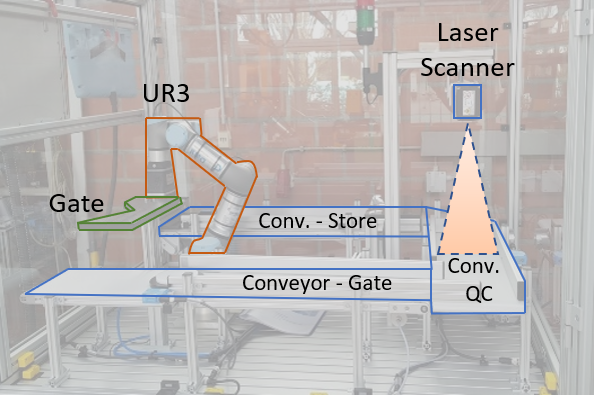
\includegraphics[width=.45\textwidth]{img/demozelle}
       \caption{The industry 4.0 demonstration cell at the University of Siegen}
\label{fig:ind_cell}
\end{figure}

\section{Machine Learning Methods} \label{sec:ML} %3/4 Page

To study which implementation would be more suitable for industrial applications, we compare Multilinear Perceptrons (MLPs), Support Vector Machines (SVM), as well as random forests on the task of quality prediction. All three will be introduced next.

\subsection{Multilayer perceptrons}
These feedforward neural networks typically combine multiple layers
and activation functions \cite{bishop2006pattern}.
A layer contains a large weight matrix and
a bias vector. To evaluate the layer the input vector must be
multiplied with the weight matrix before the bias vector is added.
Each layer is typically followed by an activation function 
which adds non-linearity to the network graph. Rectified linear units
(ReLUs) are zero for negative inputs leave positive inputs unchanged.
ReLUs are the recommended activation function for modern neural
networks \cite{goodfellow2016deep} we use these here as well.
Since the linear parts of the ReLU and the linear matrix multiplication
are differentiable we can employ gradient descent to train our 
classifier.

\subsection{Support Vector Machines}
Support Vector Machines (SVM) attempt to separate data
along hyperplanes \cite{aggarwal2015data}. 
SVM offer a convex alternative to MLPs \cite{Suykens2002least}.
A convex classifier is guaranteed to converge to a global solution
regardless of its initialization.
Non-separable data can become separable if projected to a different
possibly high dimensional space through a Kernel function.
The Kernel trick allows SVM to solve some non-linear
classification problems \cite{Suykens2002least}.
Radial basis functions (RBF) are commonly chosen as kernels
\cite{Suykens2002least}, therefore, we choose to follow this practice as well.

\subsection{Decision Tree}
Decision trees are essentially binary trees, which work with the input
features at the roots, decisions are made by moving
up the tree to top leaves. At every branch in the tree, a decision
is made, until one arrives at the decision \cite{Marsland2015Machine}.
For numerical input features, each decision partitions the data
\cite{aggarwal2015data}. For example by comparison to a threshold value.
To construct the tree these cutoff values have to be chosen at every branch. The construction problem turns into an optimization problem when a split criterion is introduced. Common choices are cross-entropy of Gini-coefficient \cite{aggarwal2015data}.
During construction, the chosen function must be minimized. 


\section{Experiments} \label{sec:experiment}

\subsection{Data acquisition}

Industrial projects require to work with a variety of sensors and controllers. Thus, there is a risk of incompatibility between technologies. To avoid that problem, universal protocols are often implemented at industrial projects. This is the case for our industry 4.0 demonstration cell, which shares data via the protocol OPC-UA. 

Figure~\ref{fig:robot_pos_cell} describes a simplified version of the real connection diagram of the demonstration cell. For our case, the data is acquired independently from two OPC-UA servers. This represents the interaction between multiple servers in real production environments. 

In our implementation, we acquired the data in two steps.
The first step consisted of listing all the variables of interest and mapping their source. The second step was to determine the use cases of interest. Our study focussed on the data described in Table.~\ref{tab:data_source} and the six use cases described in Table.~\ref{tab:use_cases}. The data was manually collected by using the software "UAExpert - v1.5.1". Approximately 15 hours of data were collected, while equally sampling each use case during the data acquisition time.

\begin{table}
       \centering
       \begin{adjustbox}{width=.45\textwidth}
       \begin{tabular}{ c c c } \toprule
              \textbf{Data of interest} & \textbf{Server Source} & \textbf{Variable}\\ \midrule
              Conveyor speed       & Siemens PLC       & \begin{minipage}[t]{0.2\textwidth}
              \begin{description}
                     \item Conveyor: Gate
                     \item Conveyor: QC
                     \item Conveyor: Store
                     \end{description}
                     \end{minipage} \\ \hline
              UR3 Position         & Siemens PLC       & \begin{minipage}[t]{0.2\textwidth}
              \begin{description}
                     \item $xyz$ Gripper position
                     \end{description}
                     \end{minipage} \\ \hline
              Action Flags         & Siemens PLC       & \begin{minipage}[t]{0.2\textwidth}
              \begin{description}
                     \item UR3 gripper open/close
                     \item Grab/drop disk based on disk type
                     \end{description}
                     \end{minipage} \\ \hline
              Quality control      & SICK SIM4000      & \begin{minipage}[t]{0.2\textwidth}
              \begin{description}
                     \item OK-NOK label
                     \item $xy$ disk deviation from the center point
                     \item Absolute disk deviation
                     \end{description}
                     \end{minipage} \\ \hline
              Gate position        & SICK SIM4000      & \begin{minipage}[t]{0.2\textwidth}
              \begin{description}
                     \item Position
                     \item Speed
                     \item Safe to go
                     \end{description}
                     \end{minipage} \\ \hline
              Store       & SICK SIM4000      & \begin{minipage}[t]{0.2\textwidth}
                     \begin{description}
                     \item Disk Size
                     \end{description}
                   \end{minipage} \\ \bottomrule
       \end{tabular}
       \end{adjustbox}
       \caption{Industry 4.0 demonstration cell: Relevant data linked with its reference source server.}
       \label{tab:data_source}
\end{table}

\begin{table}
       \centering
       \begin{tabular}{ c c } \toprule
              Use Case        & Description \\ \midrule
              Use Case 1  & \begin{minipage}[t]{0.25\textwidth}
                            \begin{description}
                                   \item Conveyor speed: Slow
                                   \item Robot position: OK
                            \end{description}
                            \end{minipage}  \\ \hline
              Use Case 2  & \begin{minipage}[t]{0.25\textwidth}
                            \begin{description}
                                   \item Conveyor speed: Slow
                                   \item Robot position: NOK
                            \end{description}
                            \end{minipage}  \\ \hline
              Use Case 3  & \begin{minipage}[t]{0.25\textwidth}
                            \begin{description}
                                   \item Conveyor speed: Fast
                                   \item Robot position: OK
                            \end{description}
                            \end{minipage}  \\ \hline
              Use Case 4  & \begin{minipage}[t]{0.25\textwidth}
                            \begin{description}
                                   \item Conveyor speed: Fast
                                   \item Robot position: NOK
                            \end{description}
                            \end{minipage}  \\ \hline
              Use Case 5  & \begin{minipage}[t]{0.25\textwidth}
                            \begin{description}
                                   \item Conveyor speed: Too Fast
                                   \item Robot position: OK
                            \end{description}
                            \end{minipage}  \\ \hline
              Use Case 6  & \begin{minipage}[t]{0.25\textwidth}
                            \begin{description}
                                   \item Conveyor speed: Too Fast
                                   \item Robot position: NOK
                            \end{description}
                            \end{minipage}  \\ \bottomrule
       \end{tabular}
       \caption{Industry 4.0 demostration cell: Controlled Use-Cases.
       Use-Cases with the value \textit{Robot position: NOK} and \textit{Conveyor speed: Too Fast} will result in NOK pieces.}
       \label{tab:use_cases}
\end{table}


\begin{figure}
       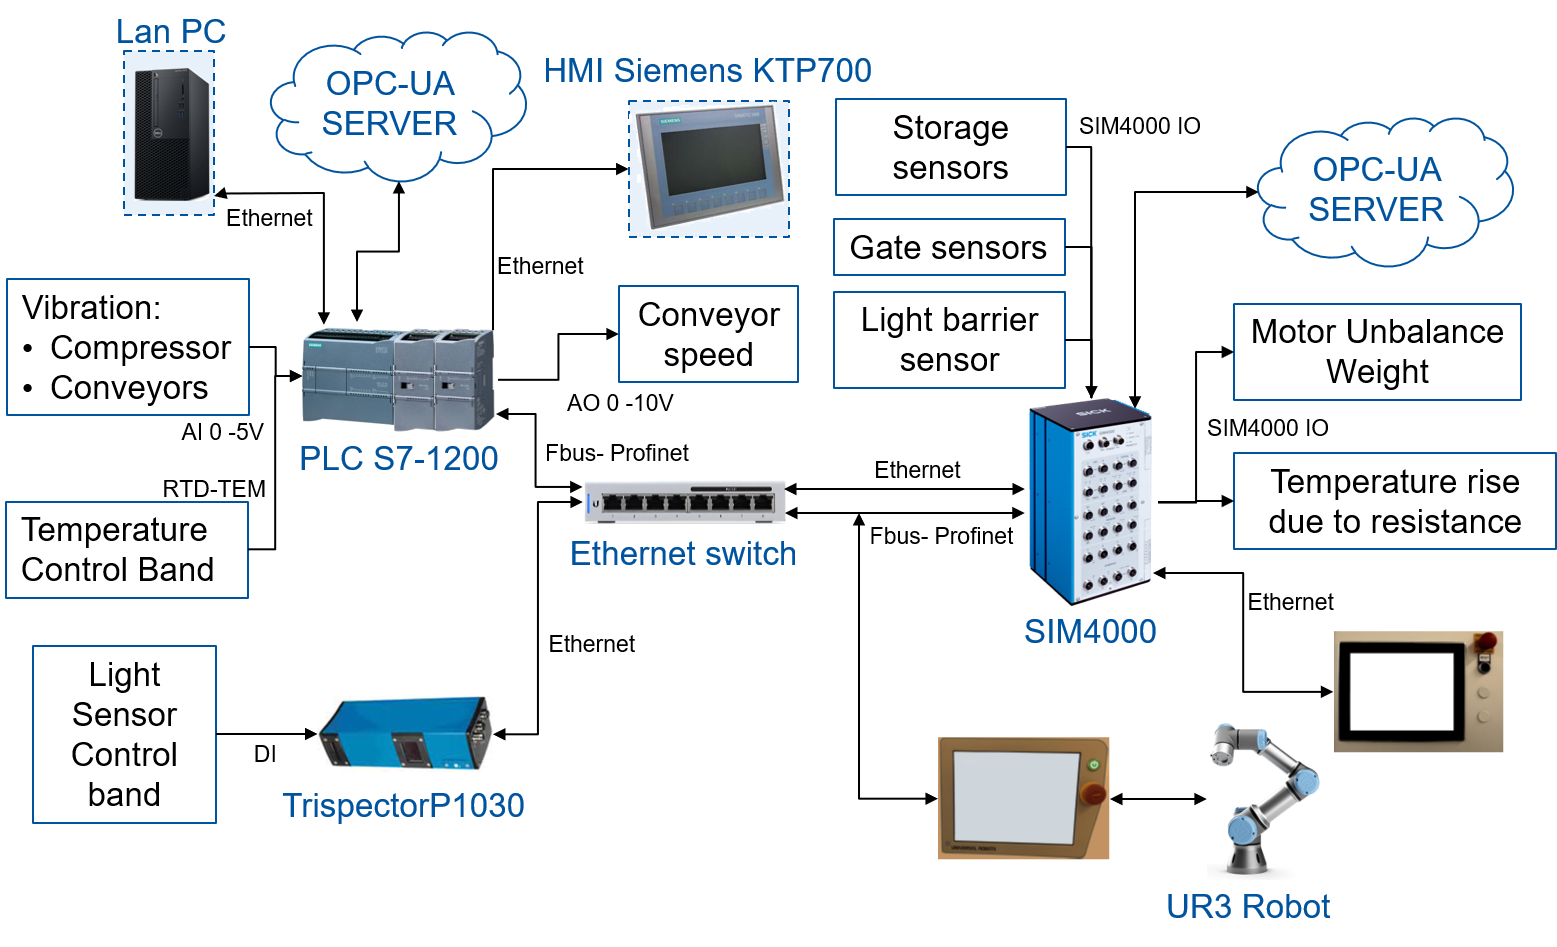
\includegraphics[width=.45\textwidth]{img/demozelle_conex_diagram.png}
       \caption{Industry 4.0 demostration cell: Connection diagram (simplified).
             }
\label{fig:demo_conn_diag}
\end{figure}

\subsection{Data preprocessing}

Once enough data is collected, the next step is to clean the raw data and organize it accordingly \cite{goodfellow2016deep}. For our case, that means to merge the data collected from the two OPC-UA servers, and synchronize the time-stamp. Since our systems are not completely synchronized, it was needed to calculate the delta-time between servers by referencing each server's base clock. Once the delta-time was determined, a time-stamp function was implemented to correct the time-shift between samples and be able to merge all the data without incompatibilities.

Data tags interpretation is an important step in the preprocessing process \cite{goodfellow2016deep}. The raw data collected from the sensors is usually tagged by an alphanumeric code predefined by the sensor manufacture. To work with the data, it was needed to implement diverse functions which have the task to clean the raw data in a more human-readable form. This means to remove samples out of clear boundaries and missing values, as well as to translate the sensor code tags based on a dictionary predefined by the authors. This last step, might be optional in other implementations, however, it proves to be a great addition for testing purposes.

Once the data is clean and compiled in one directory, our step was to split the data based on the assembly cycle. For our purpose, we split the dataset into individual data-samples with help of the action tags included in the dataset Table.~\ref{tab:data_source}. Subsequently, each data-sample is automatically checked for missing sensor values and discarded if so. At this point, we have a series of data-samples based on time series. However, we are not interested in a time series analysis, since having the time parameter would not neccesarily improve the prediction results, but rather make the approach more complex and more data would be needed, therefore it was needed to compress each time-series based data-sample in an atemporal data-sample.
To eliminate time as a variable in our dataset, we defined a series of rules to be applied in each assembly cycle data-sample:

\begin{itemize}
       \item Value of the robot position ($xyz$) while dropping the disk in the storage area
       \item Mean conveyor speed value per conveyor band
       \item Absolute deviation ($xy$) value at the quality control check
       \item Absolute quality control value: OK - NOK
\end{itemize}

Each time-series sample was evaluated based on the rules stated above, and the result of each evaluation was considered as our atemporal data-sample, which we used as the base for our classifier.

\subsection{Classifier optimization and testing}\label{sec:ml_exp}

\begin{figure}
       \includestandalone[width=.45\textwidth]{img/arm_data_plot}
       \caption{Robot arm movement patterns. We show the movement of the 
                cell's robot arm, its grippers, and the encoding of the overall
                position in the system. The changes in the grip flag are triggered,
                when the gripper opens or closes. Zero indicates an open, while
                one indicates a closed gripper. The position flags marks the state
                of the cell's arm. 0 means the black disk is in store,
                one that the black disk is at the gate, two that the white disk
                is in store and three that the white disk is located at the gate.
             }
\label{fig:robot_pos_cell}
\end{figure}

The robot's position at disk drop is marked in 
Figure~\ref{fig:robot_pos_cell}. The quality prediction problem is 
framed as a classification task. The input vectors which we feed into our
classifiers consist of the arm positions at the disk drops for both
disks in three dimensions, as well as the largest recorded belt speed
of all three belts. The interpretation of the quality measurement is 
used as the training target. It can be OK or NOK which we encode as 
zero and one.

We work with a total of 528 measurements. Each containing arm and belt data
logs of individual cell run. 50 samples are set aside at random for testing 
purposes, leaving 478 training samples. The random number generator seed is
set to one to ensure the train and test set splits are identical 
for all experiments.

We compare a total of three different classifier architectures on the data.
A Support Vector Machine (SVM), a multilinear perceptron (MLP) and a Random Forest
structure. All three methods are trained using standard hyperparameters.
\footnote{To allow exact reproduction of these results source
code is available at \url{https://github.com/manubrain/Demo-Cell-Classification}}

\begin{table}
       \centering
       \begin{tabular}{ c c } \toprule
              Approach         & accuracy \\ \midrule
              Na\"ive-Baseline & 64 \% \\
              Support Vector Machine & 82 \% \\
              Multilayer Perceptron & 88 \% \\
              Decision Tree         & 98 \% \\ \bottomrule
       \end{tabular}
       \caption{Comparison of Support Vector Machine (SVM), Multilinear Perceptron and 
                Random Forest classification on our anomaly detection task. 
                The first row shows the performance of naively predicting a broken piece
                every time.}
       \label{tab:class_comp}
\end{table}

\begin{table}
       \begin{subtable}[h]{0.3\textwidth}
              \centering
              \begin{adjustbox}{width=1.6\textwidth}
              \begin{tabular}{l|l|c|c|c}
                     \multicolumn{2}{c}{}&\multicolumn{2}{c}{True Values}&\\
                     \cline{3-4}
                     \multicolumn{2}{c|}{}& OK & NOK &\multicolumn{1}{c}{Total}\\
                     \cline{2-4}
                     \multirow{2}{*}{Predicted Values}& OK & $18$ & $0$ & $18+0 = 18$\\
                     \cline{2-4}
                     & NOK & $8$ & $24$ & $8+24 = 32$\\
                     \cline{2-4}
                     \multicolumn{1}{c}{} & \multicolumn{1}{c}{Total} & \multicolumn{1}{c}{$18+8 = 26$} & \multicolumn{    1}{c}{$0+24 = 24$} & \multicolumn{1}{c}{$50$}\\
              \end{tabular}
              \end{adjustbox}
              \caption{Support Vector Machine.}
              \label{tab:SVM_conf_matrix}
       \end{subtable}
       \begin{subtable}[h]{0.3\textwidth}
              \centering
              \begin{adjustbox}{width=1.6\textwidth}
              \begin{tabular}{l|l|c|c|c}
                     \multicolumn{2}{c}{}&\multicolumn{2}{c}{True Values}&\\
                     \cline{3-4}
                     \multicolumn{2}{c|}{}& OK & NOK &\multicolumn{1}{c}{Total}\\
                     \cline{2-4}
                     \multirow{2}{*}{Predicted Values}& OK & $18$ & $0$ & $18+0 = 18$\\
                     \cline{2-4}
                     & NOK & $6$ & $26$ & $6+26 = 32$\\
                     \cline{2-4}
                     \multicolumn{1}{c}{} & \multicolumn{1}{c}{Total} & \multicolumn{1}{c}{$18+6 = 24$} & \multicolumn{    1}{c}{$0+26 = 26$} & \multicolumn{1}{c}{$50$}\\
              \end{tabular}
              \end{adjustbox}
              \caption{Multilayer Perceptron.}
              \label{tab:MPL_conf_matrix}
       \end{subtable}
       \begin{subtable}[h]{0.3\textwidth}
              \centering
              \begin{adjustbox}{width=1.6\textwidth}
              \begin{tabular}{l|l|c|c|c}
                     \multicolumn{2}{c}{}&\multicolumn{2}{c}{True Values}&\\
                     \cline{3-4}
                     \multicolumn{2}{c|}{}& OK & NOK &\multicolumn{1}{c}{Total}\\
                     \cline{2-4}
                     \multirow{2}{*}{Predicted Values}& OK & $17$ & $1$ & $17+1 = 18$\\
                     \cline{2-4}
                     & NOK & $0$ & $32$ & $0+32 = 32$\\
                     \cline{2-4}
                     \multicolumn{1}{c}{} & \multicolumn{1}{c}{Total} & \multicolumn{1}{c}{$17+0 = 17$} & \multicolumn{    1}{c}{$1+32 = 33$} & \multicolumn{1}{c}{$50$}\\
              \end{tabular}
              \end{adjustbox}
              \caption{Decision Tree.}
              \label{tab:Tree_conf_matrix}
       \end{subtable}
       \caption{Confusion matrices result of the prediction of 50 test data-points. We present the result of the predictions given by all three algorithms in detail based on the comparison between true values vs predictions. The tables read from the upper left cell as: true-positive, false-positive, false-negative, true-negative.}
       \label{tab:Confusion_matrix}
\end{table}


Results are shown in table~\ref{tab:class_comp}. For 32 of the total 50 test samples
quality measurements indicate a problem. This sets the 
baseline over the entire data set, which would be obtained by simply labeling all samples
as faulty. Over the test set, we require to classify more than 64\% of the data correctly.
We would therefore expect any naive classifier to produce at least 64\% accuracy, which we have to surpass. In Table~\ref{tab:class_comp}, we observe that this is indeed the case for all three approaches evaluated here.

Based on the MLP prediction results presented on Table.~\ref{tab:Confusion_matrix}\subref{tab:MPL_conf_matrix} shows that even though the prediction model is not 100\% accurate, the percentage of false-positive predictions is 0\%. The false-negative results represent the 12\% of the test sample and the true predictions constitute 88\% of the test data.

The outcome of the models shows that the random forest performed best followed by the multilinear perceptron and the support vector machine. However, by reviewing the confusion matrices presented in Table.~\ref{tab:Confusion_matrix}, multilinear perceptron would be the preferred solution to be implemented at industrial applications due to the 0\% ratio in false-positive results and high accuracy of 88\%.

\section{Conclusion} \label{sec:conclusion}

% Quality assurance is an important topic in production. Quality assurance methods in production might diverge one from each other, however, all of them seek to prove the product quality in one way or another. 

Based on the explorative literature review, we observed that the hundred percent quality check method proves to be the most efficient method to guarantee the final product quality, however, the high implementation cost is its biggest draw-back. On the other hand, we have the statistical methods, which are known to be fast and efficient, but the lack of reviewing each product until the next batch review might imply a considerable loss of the produced products whenever NOK products are found. This is based on the uncertainty of when did the error occur and how many products are affected.

By implementing ML models capable to predict the quality of the product, based on just the initial conditions of the process would be a great asset for the industrial processes. Within the limits of our work, we predict with 98\% certainty the product quality by implementing a decision tree model with a 6-variables vector as input. 
However, our decision for industrial applications would be the MLP with 88\% accuracy as to guarantee that all passed parts are OK and avoid labeling a NOK piece as OK. For further work, we expect to increase the accuracy of the prediction model by collecting more data-samples and experimenting with other, more complex, ML models.

It is important to state that this prediction model is not yet ready to fully replace the statistical methods, not the hundred percent quality check method, since this research is still on its early stages and need further development. However, a combination of SPC along prediction models could work well together, since the prediction model will evaluate each produced piece, and this might compensate one disadvantage of the statistical methods.

It is worth to mention the most important points learned during the project implementation. This might help as building blocks for further research in the area.

\section{Lesson Learned} \label{sec:lessons} % 1/2 Page

\textbf{Incompatibility between technologies}; devices configured on the same network presented troubles to share data due to network restrictions, as well as the limitation to access and modify restricted program-code given by the machine manufacture. 
To overcome the situation stated above, it was necessary to reprogram big sections of the machine control system.

\textbf{Data synchronization}; two OPC-UA servers were used on this implementation. This lead to a series of data synchronization problems due to differences in the internal clock of both servers.
To solve the issue, it was needed to write a time-stamp synchronization script that was deployed during the data preprocessing phase. Without harmonious time-stamps, determining the production cycle would have been impossible and the input data for the ML model would have been useless, and the model inaccurate. 

\textbf{Data interpretation}; this process is considered complicated, time-consuming, and a fundamental step for any ML applications. It is fundamental to understand the assembly process, the timing from the machine movements, the boundaries of the machine's sensors, as well a basic correlation within the presented data.

\textbf{Missing values}; to minimize the risk of false results delivered by the ML model, it would be compulsory to carefully review the ML input data. Missing values can have a great impact on the ML prediction, that is the reason why we deliberately review all the input data and validate it with the expected output from the diverse sensors. Whenever there was missing data, and as long as we did not fabricate data, we employed statistical methods to fill the data gap.

\textbf{Adapting the industry 4.0 demonstration cell}; the initial state of the demonstrator was very limited. Even though the process was well known, the lack of labels or flags whenever certain actions occur, made it complicated to have accurate data sampling from each assembly cycle. To overcome this uncertainty, we modified the machine program to raise specific flags whenever certain actions were executed.

\textbf{Machine Learning}; careful measurement and  meaningful preprocessing
of our cell-data was key to the successful application of all three algorithms.
Without the labels, the problem could not have been framed as a supervised 
classification problem.

\textbf{Dataset size}; as the starting point we collected as many data points as the ones found in the iris Dataset \cite{fisher_1936}. The next step was to collect batches of data of around 30 minutes per use case. This process was repeated until accumulate around 15 hours of data.

\section*{Acknowledgments}
This work was funded by the European Regional Development Fund (ERDF) within the project "ManuBrain".

\bibliographystyle{elsarticle-harv} %elsarticle-harv} %abbrv %IEEEtran
\bibliography{bib}

\end{document}
